\documentclass[a4paper,11pt]{jsarticle}


% 数式
\usepackage{amsmath,amsfonts,amssymb}
\usepackage{bm}
% 画像
\usepackage[dvipdfmx]{graphicx}
\usepackage[dvipdfmx]{color}
\usepackage{siunitx}
\usepackage{wrapfig}
\usepackage{cases}
\usepackage{dcolumn}
\usepackage{subcaption}
\makeatletter
\newcommand{\figcaption}[1]{\def\@captype{figure}\caption{#1}}
\newcommand{\tblcaption}[1]{\def\@captype{table}\caption{#1}}
\makeatother

\usepackage{listings,jvlisting}
\lstset{
basicstyle={\ttfamily},
identifierstyle={\small},
commentstyle={\smallitshape},
keywordstyle={\small\bfseries},
ndkeywordstyle={\small},
stringstyle={\small\ttfamily},
frame={tb},
breaklines=true,
columns=[l]{fullflexible},
numbers=left,
xrightmargin=0zw,
xleftmargin=3zw,
numberstyle={\scriptsize},
stepnumber=1,
numbersep=1zw,
lineskip=-0.5ex
}

\begin{document}

\title{衝突前後の運動方程式について}
\author{平林広}
\date{\today}
\maketitle

今回の文書の目的は
衝突によって物理量の変化が想像しづらい場合において
どのように衝突を考えるべきかをまとめることである。

\section{重力下での煙突方向衝突}
まずは慣れ親しんだ衝突から
加速度や力といった2階微分の物理量以外は衝突において無視してよいことを学ぶ。

\begin{figure}[h]
  \centering
  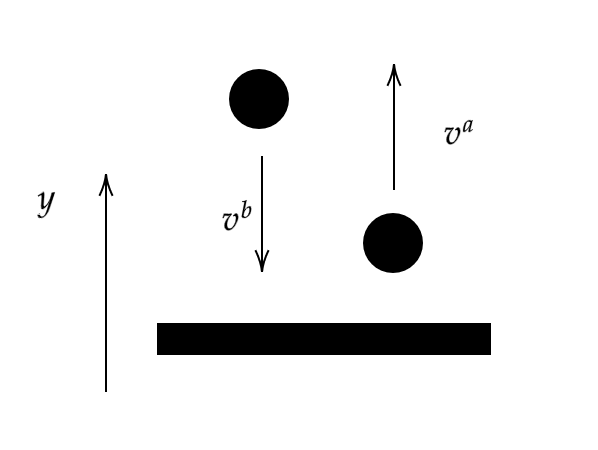
\includegraphics[width = 0.6\textwidth]{ball_freefall.png}
  \caption{衝突状況}
  \label{ball_freefall.png}
\end{figure}

質点$m$が鉛直方向のみに運動し、
地面に速度$v^b (b\text{はbeforeの意図})$ で衝突し、
速度$v^a (a\text{はafterの意図})$で跳ね上がる場合を考える。
ただし、ここで$v^a$は未知である、という考えておく。

衝突は$t=0$で起きるように時刻$t$を取る。
運動方程式は地面からの力を$F$として
\begin{align*}
  m a = -mg + F
\end{align*}
とあらわされる。ただし$F$は以下程度にしか分からない。
\begin{align*}
  F = \begin{cases}
    \infty & (t = 0)
    \\
    0 & (t \neq 0)
  \end{cases}
  .
\end{align*}

区間$[-t_1, t_1]$での積分を考える。
\begin{align*}
  \int_{-t_1}^{t_1} m a dt = \int_{-t_1}^{t_1} -mg dt + \int_{-t_1}^{t_1} F dt
  .
\end{align*}
$t_1 \rightarrow 0$の極限をとれば、$F$による力積を$L$として、
\begin{gather*}
  \int_{-t_1}^{t_1} m a dt \rightarrow m(v^a - v^b),
  \int_{-t_1}^{t_1} -mg dt \rightarrow 0,
  \int_{-t_1}^{t_1} F dt = L
\end{gather*}
となるから、
衝突の前後において
\begin{gather}
  m(v^a - v^b) = L
  \label{case1:newton}
\end{gather}
となる。
しかし現時点では未知数が$v^a, L$に対して、方程式が1つであるため、解けない。

そこで、衝突の条件を考える。
弾性係数を$e$とすると、
\begin{gather}
  v^a = -e v^b
  \label{case1:collision}
\end{gather}
という方程式が導かれる。

よって Equation \ref{case1:newton}, \ref{case1:collision}により
\begin{align*}
  \begin{cases}
    m(v^a - v^b) &= L
    \\
    v^a = -e v^b
  \end{cases}
\end{align*}
と、未知数が$v^a, L$に対して、方程式が2つ成り立つため、
$v^a, L$を決定することができる。

\section{単振り子の衝突}

\section{2重振り子の衝突}

\end{document}